% Auto-generated by scripts/package_update_frequency_paper_assets.py
\begin{figure}[t]
  \centering
  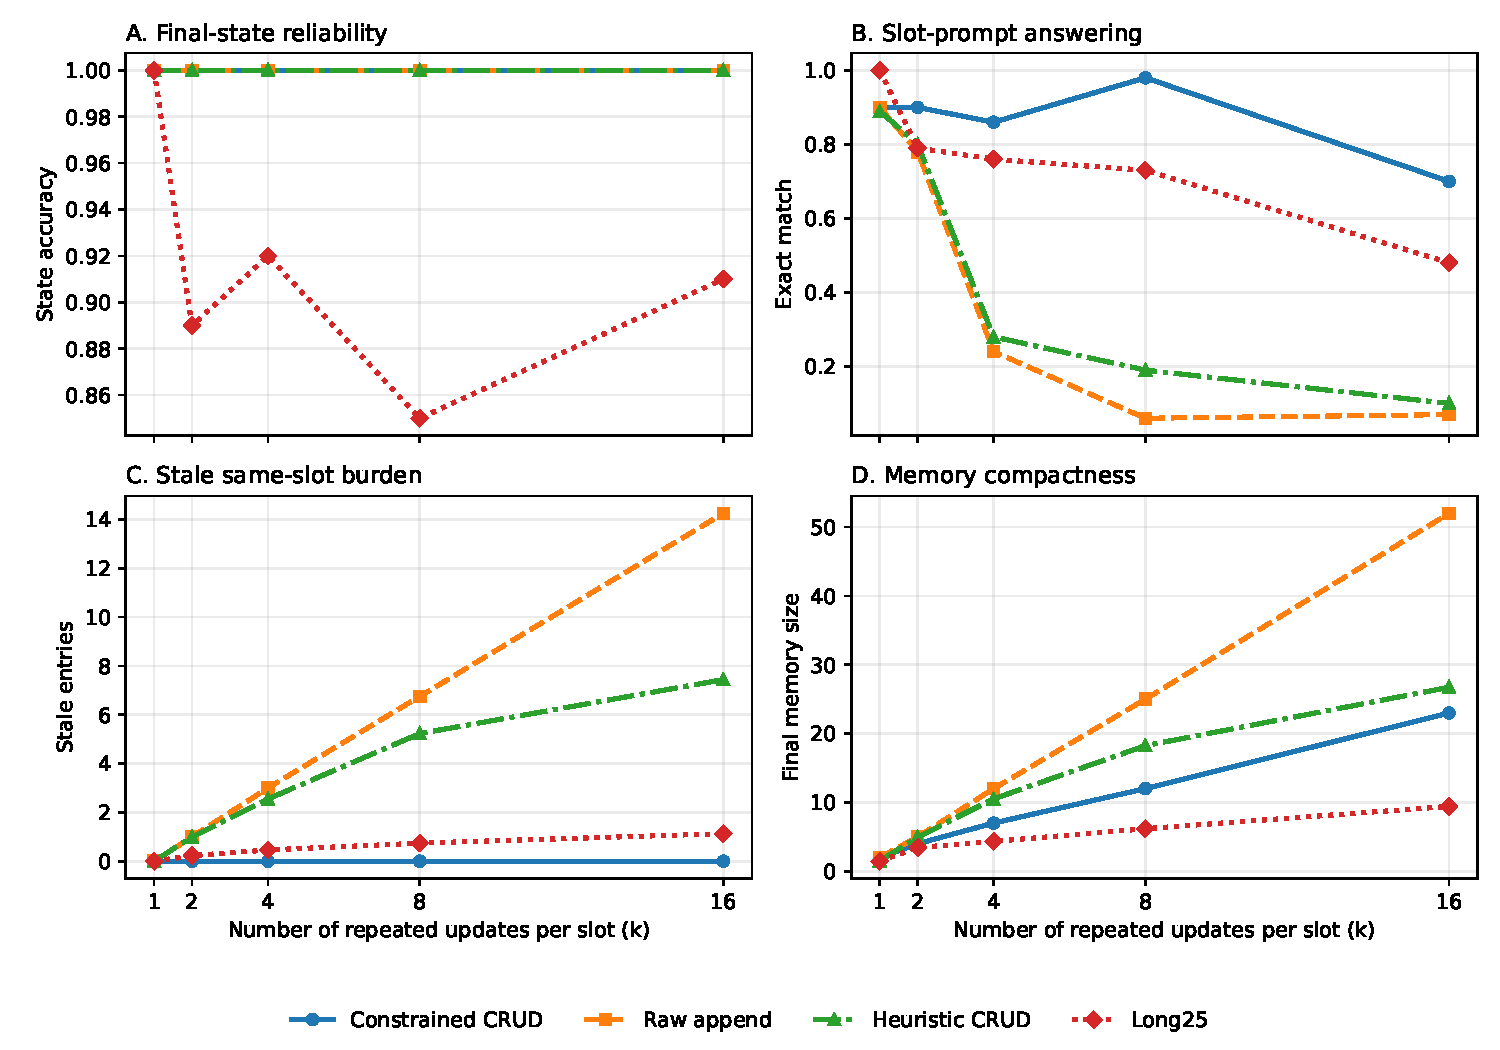
\includegraphics[width=0.95\linewidth]{paper/p63_update_frequency_tradeoff.pdf}
  \caption{Update-frequency stress test on P6.3 hard splits. Oracle-like slot-direct state evaluation hides stale-memory burden for append-only and heuristic methods, while slot-prompt answering reveals answer collapse as repeated same-slot updates accumulate stale entries. Long25 is substantially more compact but sacrifices final-state reliability under hard distractors.}
  \label{fig:p63-update-frequency-tradeoff}
\end{figure}

\begin{table}[t]
  \centering
  \small
  \begin{tabular}{lcccc}
    \hline
    Method & State acc. & EM/F1 & Stale & Mem. size \\ 
    \hline
    Constrained CRUD & 1.00 & 0.70 / 0.70 & 0.00 & 23.00 \\
    Raw append & 1.00 & 0.07 / 0.10 & 14.25 & 52.00 \\
    Heuristic CRUD & 1.00 & 0.10 / 0.13 & 7.44 & 26.73 \\
    Long25 & 0.91 & 0.48 / 0.53 & 1.13 & 9.43 \\
    \hline
  \end{tabular}
  \caption{k=16 tradeoff among final-state reliability, slot-prompt answer quality, stale same-slot burden, and memory compactness. Append-only and heuristic managers preserve slot-direct recoverability but collapse under slot-prompt answering; Long25 is compact but not fully reliable.}
  \label{tab:p63-k16-tradeoff}
\end{table}

% Derived diagnostic figures
\begin{figure}[t]
  \centering
  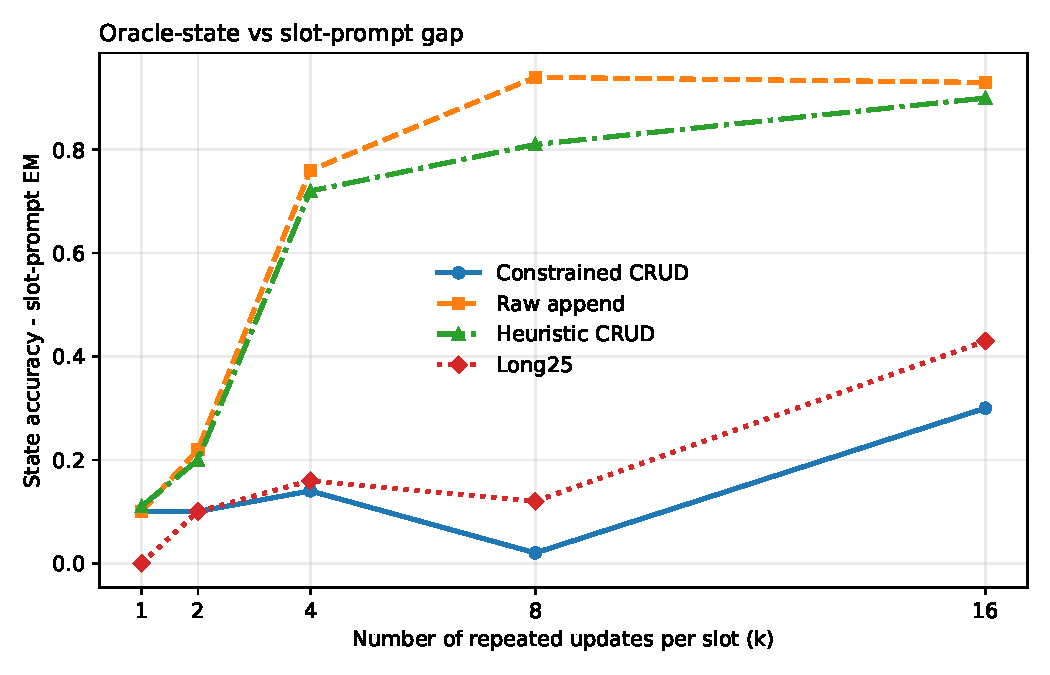
\includegraphics[width=0.78\linewidth]{paper/p63_gap_slot_direct_vs_prompt.pdf}
  \caption{Gap between oracle-like slot-state accuracy and slot-conditioned exact match across update frequencies. Larger gaps indicate cases where final-state recoverability is preserved while realistic answering degrades.}
  \label{fig:p63-direct-prompt-gap}
\end{figure}

\begin{figure}[t]
  \centering
  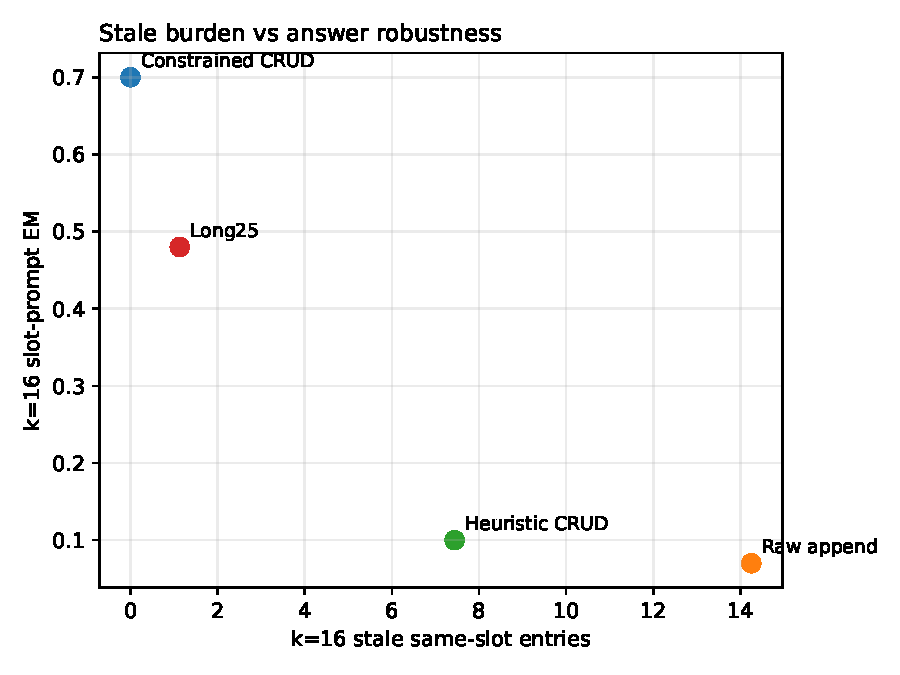
\includegraphics[width=0.78\linewidth]{paper/p63_stale_vs_prompt_em_k16.pdf}
  \caption{At k=16, stale same-slot burden is strongly associated with lower slot-conditioned exact match. This view highlights stale evidence as the main failure pressure for append-only and partial-compaction methods.}
  \label{fig:p63-stale-vs-em}
\end{figure}

\begin{figure}[t]
  \centering
  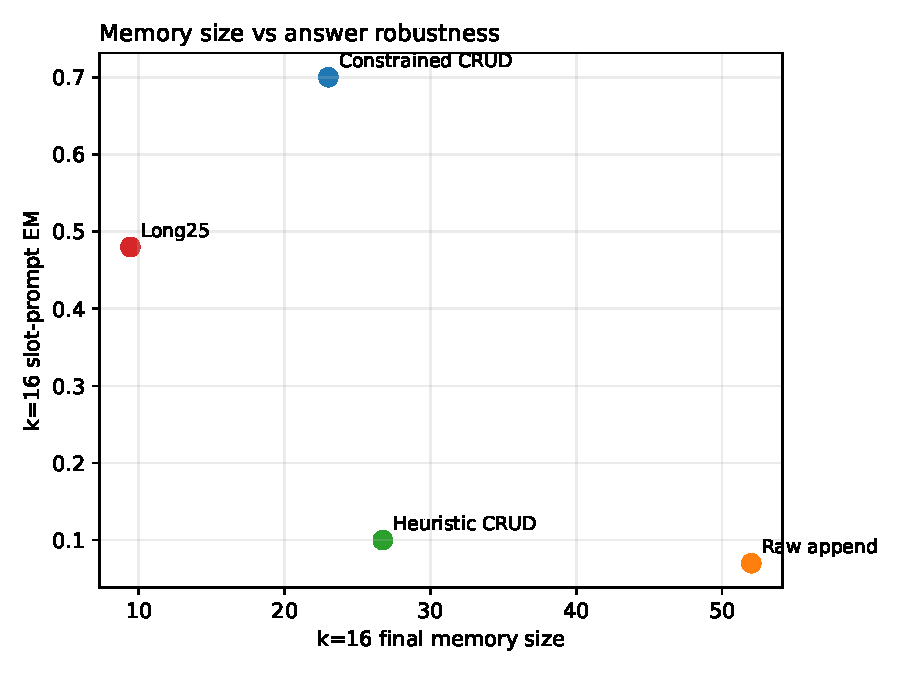
\includegraphics[width=0.78\linewidth]{paper/p63_memory_size_vs_prompt_em_k16.pdf}
  \caption{At k=16, final memory size and slot-conditioned exact match expose the compactness--robustness frontier. Long25 is compact but imperfectly reliable, while append-only memory is large and brittle under prompting.}
  \label{fig:p63-size-vs-em}
\end{figure}

% Appendix-ready k-sweep tables
\begin{table}[t]
  \centering
  \small
  \begin{tabular}{lccccc}
    \hline
    Method & k=1 & k=2 & k=4 & k=8 & k=16 \\ 
    \hline
    Constrained CRUD & 1.00 & 1.00 & 1.00 & 1.00 & 1.00 \\
    Raw append & 1.00 & 1.00 & 1.00 & 1.00 & 1.00 \\
    Heuristic CRUD & 1.00 & 1.00 & 1.00 & 1.00 & 1.00 \\
    Long25 & 1.00 & 0.89 & 0.92 & 0.85 & 0.91 \\
    \hline
  \end{tabular}
  \caption{Slot-direct state accuracy across update frequencies.}
  \label{tab:p63-slot-direct-sweep}
\end{table}

\begin{table}[t]
  \centering
  \small
  \begin{tabular}{lccccc}
    \hline
    Method & k=1 & k=2 & k=4 & k=8 & k=16 \\ 
    \hline
    Constrained CRUD & 0.90/0.91 & 0.90/0.94 & 0.86/0.86 & 0.98/0.98 & 0.70/0.70 \\
    Raw append & 0.90/0.91 & 0.78/0.79 & 0.24/0.27 & 0.06/0.10 & 0.07/0.10 \\
    Heuristic CRUD & 0.89/0.91 & 0.80/0.81 & 0.28/0.28 & 0.19/0.22 & 0.10/0.13 \\
    Long25 & 1.00/1.00 & 0.79/0.79 & 0.76/0.77 & 0.73/0.74 & 0.48/0.53 \\
    \hline
  \end{tabular}
  \caption{Slot-prompt EM/F1 across update frequencies.}
  \label{tab:p63-slot-prompt-sweep}
\end{table}

\begin{table}[t]
  \centering
  \small
  \begin{tabular}{lccccc}
    \hline
    Method & k=1 & k=2 & k=4 & k=8 & k=16 \\ 
    \hline
    Constrained CRUD & 0.00 & 0.00 & 0.00 & 0.00 & 0.00 \\
    Raw append & 0.00 & 1.00 & 3.00 & 6.75 & 14.25 \\
    Heuristic CRUD & 0.00 & 1.00 & 2.55 & 5.23 & 7.44 \\
    Long25 & 0.00 & 0.23 & 0.46 & 0.74 & 1.13 \\
    \hline
  \end{tabular}
  \caption{Stale same-slot entries across update frequencies.}
  \label{tab:p63-stale-sweep}
\end{table}

\begin{table}[t]
  \centering
  \small
  \begin{tabular}{lccccc}
    \hline
    Method & k=1 & k=2 & k=4 & k=8 & k=16 \\ 
    \hline
    Constrained CRUD & 2.00 & 4.00 & 7.00 & 12.00 & 23.00 \\
    Raw append & 2.00 & 5.00 & 12.00 & 25.00 & 52.00 \\
    Heuristic CRUD & 1.50 & 4.97 & 10.51 & 18.25 & 26.73 \\
    Long25 & 1.46 & 3.45 & 4.34 & 6.18 & 9.43 \\
    \hline
  \end{tabular}
  \caption{Final memory size across update frequencies.}
  \label{tab:p63-memory-size-sweep}
\end{table}
